\chapter{Introduction}
\label{chapter:introduction}
\index{Introduction}

%aforementioned
\section{Motivation}
Over the past decade rapid rise of creating data in all areas of society such as traffic, medicine, social network,industry, etc, has highlighted the need for enhancing the process of analyzing this data. \textit{Big Data} is the the approach when it is analyzed an extremely large data. One of the main reasons why Big Data has emerged, is the fact that, classical algorithms are not able to manage this amount of data because when they were designed this problem was unimaginable.
%amount of data

Currently optimization problems are not unrelated to this trend, hence multi-objective optimization algorithms (MOOA) must take into account this new scenario, which means that,  MOOAs have to face with either various data sources or huge amount of data, this features are found in dynamic multi-objective Big Data problems (DMOPs).
When dealing with DMOPs, whenever there exist changes in the environment that affect the solutions of the problem (i.e.,\ the Pareto set, the Pareto front, or both), therefore in the fitness landscape, the optimization algorithm must react to adapt the search to the new features of the problem~\cite{FDA04}. This means that a dynamic multi-objective optimization metaheuristic must be able to detect when the problem changes and to apply a strategy to cope with the changes, so that means that, they have to be interactive with the context \cite{lopez2015machine}.

A decision maker(DM) is a person who is an expert in the domain of the multi-objective optimization problem and can express his/her preference information to choose a single, the most preferred solution.
DM reaches a decision to choose between multiple criteria about the problem, usually which are in conflict, in order to select the preferred solution, this kind of multi-objective approach is named multiple criteria decision making (MCDM).

DM's preferences can be included in interactive multi-objective algorithms through different preference information modeling \cite{greco2005multiple} \cite{purshouse2014review}, nevertheless, in this tesis we have modeling this information through \textit{reference points} thus this way is the most popular in practice when we are working with real world problems.

%this kind of multi-objective optimization is called multiple criteria decision making (MCDM).

%Although the main goal of multi-objective optimization metaheuristics is to find a set of non-dominated solutions with the features of convergence and diversity with respect to the Pareto front of the problem at hands, however from a practical point of view, the ultimate goal when solving any MOP (static or dynamic) is to identify a feasible solution which is the most preferred for a decision maker(DM). 
%DM reflects their multiple preferences through reference point to the MOOA and this fact affects  hence, \textit{Multi criteria decision making} (MCDM) process can be applied to multi-objective Big Data problems.


%To this end, a Pareto front approximation can be of great help, since it gives information about the problem itself (i.e.,\ the ranges of the objective functions and the conflict degree among them). However, selecting the most preferred Pareto optimal solution, analyzing and comparing a large number of solutions at the same time may be cognitively demanding for the DM, especially in the presence of many objectives. Indeed, it may be computationally expensive to generate a large number of solutions approximating the whole Pareto front, particularly when dealing with real-life problems, which may even be a wasted effort if the DM is interested in just a subset of solutions located in a particular region.

%workflow
A Big Data analytics is long and complex process therefore, is carried out through a series of steps, a typical analysis is compound of data collection, data manipulation, data analysis and data visualization, hence, \textit{workflows} are useful when a process is made up of tasks.

%the follow operations,  data collections of the different data sources, manipulating  so as to prepare the data  for the analysis, analyzing and as the last step, display the analysis' result so, workflows are become useful in this kind of analysis.

The process of creating a workflow requires that the analyst takes into account the semantic and the domain of the problem and its data, as well as, the semantic of the algorithm, which is used to resolve it. Ontology is the standard way for describing the knowledge about a domain, therefore, the description of the domain of Big Data analysis such as, problems, data, algorithms, workflows, etc, is carried out using an ontology.
As mentioned above, the process of developing a workflow is not trivial, so an analyst who barely knows the different type of algorithm for analyzing data (optimization, data mining, deep learning, etc) can have problem in the moment of choosing them, so, an ontology, which has all this knowledge, will be a useful help in the process of designing new workflows.

As a global target of this PhD Thesis, we are interested in investigating the use of the semantic in the process of Big Data analysis, not only in Machine Learning analysis but also optimization. 
We define a workflow so as to analyze a Big Data problem with the help of the semantic. 
In Figure \ref{fig:conceptual_cloud} illustrates the conceptual cloud involving the Big Data analysis that we have covered in this thesis. Finally, as a product, all that work has also led the development of a software in the scope of jMetalSP library, aimed at supporting the design and development of dynamic metaheuristics for solving Big Data optimization problems. In addition, the ontology BIGOWL has been developed which defines all the components used in a Big Data analysis, from gathering data to showing the analysis result.
Finally, a number of realistic problem instances, simulation rule files, software scripts, and free web sites have been generated and are available.
%hablar de la complejidad de la creación de un worklfoew y decir que con la tecnología de web semantic podemos facilitar el uso del diseño de un workflow
%WEb semantic

%Hence, classical approach  
%aplicaciones reales, streaming
%optimisation
%web semantic
%workflow
%decision maker
%\vspace{0.5cm}
%[width=0.80\textwidth]

\begin{figure}[H] %tb
\label{fig:conceptual_cloud}
	\vspace{0.5cm} \centering 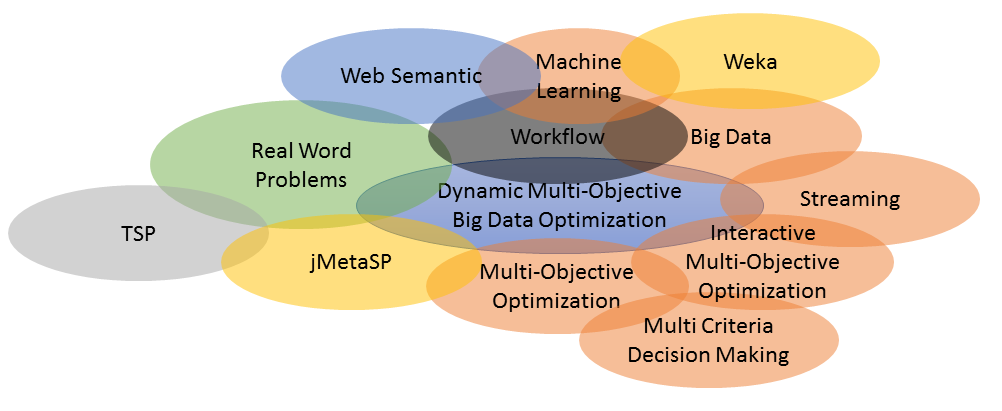
\includegraphics[width=0.95\textwidth]{figures/introduction/conceptual-model.png}
	\caption{Optimization techniques classification.}\label{fig:OptTechClass} \vspace{0.5cm}
\end{figure}



\section{Objectives and phases}
This PhD thesis focuses on analyzing the optimization in Big Data problems, as well as the benefits of making use of the semantic in the process of developing a workflow. 
For the sake of clarity, we sum up the main contributions of this thesis as follows:
\begin{itemize}
\item Analyze current state of Big Data Optimization and identify the most important deficiencies it shows on complex optimization.
%estado actual del análisis del big data e identtificar deficiencias
\item Design of new Big Data optimization proposal by means of managing dynamic changes on the Big Data problems, deal with different data source, most of them streaming and apply interactive multi-objective optimization methods in Big Data optimization.
\item Analyze current ontology versions in the process of design workflows and identify their deficiencies. 
%analizar el uso de la semántica para su uso en el análisis del big data
\item Validate our findings in previous points for solving real-world problems.
\item Develop innovative approaches that enhance the performance of current Big Data optimization techniques from the perspective of the quality of the solutions produced, or from the perspective of the computational effort required to reach them. Demonstrate their effectiveness through statistically assessed experimental evaluation.

%validación de lo anterior con casos de uso del mundo real
\end{itemize}



\section{Thesis contributions}
\label{sec:introduction-contributions}

To summarize, the main contributions of this thesis are shown below:

\begin{itemize}
	\item This thesis addresses a key challenge nowadays, that is to adapt current metaheuristics to cope with Big Data optimization \cite{BD-challenges-2014}]. As a result, we have developed jMetalSP, which is a Big Data optimization framework. 
    \item Include semantic in the design of workflow whose aim is to indicate the steps so as to analyze a Big Data problem. As a result, BIGOWL ontology has been created. 
    \item We are aimed at solving real world complex problems with dynamic multi-objective  algorithms . In concrete, we have focused in this thesis on traffic problem
    \item We have designed and developed interactive multi-objective methods (iEMO) such as inDM2[referencia] and SMPSO/RF[referencia] in order to, iEMO meets Big Data optimization. 

\end{itemize}


\section{Thesis organization}

This thesis has been organized as follows.
The current chapter contains an introduction to the work done, presenting the motivation to carry it out, the objectives that have been sought, the phases that have been followed to achieve those objectives and the main contributions of the thesis.
Chapter~\ref{chapter:multiobjective} focuses on describing the principles about the multi-objective optimization algorithms that have been used to tackle Big Data optimization problems. 
Chapter~\ref{chaper:jmetalsp} includes a full description about the framework which has been developed for optimizing Big Data optimization problem in this the. 
%Chapter~\ref{chapter:methodology} includes all the methodology that was applied in this thesis: we have included technical specification of AutoDock, jMetal framework and the integration followed of these tools to carry out the experiments.
Chapter~\ref{chapter:publishedWorks} contains all the published work that supports this thesis with a summary of each one of them.
%Chapter~\ref{chapter:results} shows a global summary of the results obtained in the published work for the mono-objective and multi-objective studies.
Finally, Chapter~\ref{chapter:conclusions} includes the conclusions of this dissertation and the future research lines that can be opened by this study.






















%\noindent La ingeniería civil es una disciplina que se ocupa del diseño, construcción y mantenimiento de obras edilicias, viales, hidráulicas, etc. cuyos proyectos se materializan como obras en lugares definidos con cierto destino y para algún fin determinado \citep{ICE12}. Entre estos tipos de obras podemos nombrar a los puentes, carreteras, túneles, canales, embalses para la regulación de ríos y para la generación de energía eléctrica, acueductos, redes de agua, edificios y torres, naves para plantas industriales, etc. Concretar alguna de estas obras requiere contar con materiales industrializados de producción a gran escala, para lo cual entre otros se necesita materia prima como la madera, minerales, rocas, etc. Los materiales utilizables y disponibles al pie de la obra pasan por una serie de procesos y etapas que van desde la extracción, industrialización, comercialización y distribución. Algunos de estos procesos para obtener el material producen degradación de la superficie y contaminación del medio ambiente, cambiando el paisaje o peor aún dejando huellas permanentes en el planeta que tal vez sean contraproducentes para los seres vivos. Cada parte o ítem que conforma una obra civil debería tener bajo impacto ecológico si los materiales se utilizaran racionalmente. Ajustar las cantidades de materiales en obras civiles con óptica económica garantizando la seguridad y sin poner en riesgo la construcción, es tarea del ingeniero proyectista.
%
%
%\vspace{-0.25cm}
%% Justificacion de la temática
%\section{Motivación}
%\label{section:motivacion}
%\index{Introducción!Motivación}
%
%Hay dos palabras claves que hemos utilizado en la sección anterior, cantidad y seguridad. Si nuestro proyecto no tuviera un equilibrio entre cantidad de materiales y seguridad, en pos de la seguridad se utilizaría una cantidad mayor de materiales de la necesaria, aumentando el costo del proyecto, por lo que tal vez sería inviable construirlo. Además, si éste se reproduce en otros proyectos aceleraríamos el proceso de degradación de la tierra por el aumento de la demanda de la materia prima, aumentando también la contaminación por polución y desperdicios generados por la industrialización. Si lo pensamos desde el otro punto de vista, de economizar en demasía, reduciendo la cantidad de materiales inherentes a la resistencia y estabilidad de la obra, estaríamos corriendo la línea hacia el límite del servicio aceptable o admisible y, pasado éste, aumenta el riesgo de la seguridad. La falta de materiales en lugares críticos es una de las causas del elevado costos de mantenimiento, de la falta de comodidad por vibraciones y el acortamiento de la vida útil por reducción del tiempo de durabilidad de lo edificado, imprevistos o acciones imprevisibles tal vez ocasionen colapso o excesiva deformación a temprana edad.
%
%En esta tesis se va a considerar el diseño de un tipo de construcciones civiles concreto, las estructuras civiles de barras definidas en el espacio y calculadas íntegramente como un todo y no por partes individuales. Se incluyen pero no se abordan problemas de estructuras planas (2D) o simplificaciones que opten por soluciones de elementos coincidentes con un único plano respecto a las disposiciones geométricas, las acciones y desplazamientos. En las estructuras civiles abordadas aseguramos la vida útil teniendo en cuenta la estabilidad, la resistencia y la durabilidad, contemplándose verificaciones globales, cumpliendo en parte con la seguridad del servicio de que la estructura se mantendría en pie. La seguridad de una estructura está asociada al conocimiento de la resistencia de los materiales que la constituye, a la ubicación de los volúmenes de los materiales para que resistan y absorban las cargas y esfuerzos a los que estará sometida, sin que exista posibilidad de riesgo de colapso o servicio. La seguridad que debe brindar una estructura civil incluye entre otros, el resguardo y protección de personas, animales y bienes ante acciones derivadas de los fenómenos terrestres y climáticos.
%
%La estructura de barras tiene una disposición lineal esquemática espacial, de forma esquelética o de alambre, siendo los ejes que pasan por el baricentro de la sección transversal las líneas representativas de las barras. Las barras tienen longitud fija y están unidas a otras por nodos y los nodos están definidos en el espacio por un sistema de coordenadas cartesiano de tres ejes. Estos nodos proven vinculaciones entre las barras. Los nodos y las barras tienen propiedades e identificaciones de modo tal que puedan ubicarse en el espacio y ser individualizados en la topología de la estructura. La topología es la representación esquemática del conjunto de nodos y de barras dispuestos para dar la forma esquelética de la estructura. Un ejemplo se muestra en la Figura~\ref{figure:nave}, que incluye una nave industrial.
%
%
%\begin{figure}
%\centering
%\includegraphics[width=1\textwidth]{Graphics/Estructuras/NAVE-INDUSTRIAL-VISTAS.eps}
%\caption{Ejemplo de estructura de barras: nave industrial.}
%\label{figure:nave}
%\end{figure}
%
%Entre las complejidades del diseño de estructuras está la manera en que se considera la distribución de los esfuerzos internos o dicho de otra manera, la distribución del trabajo entre las barras que interactúan solidariamente. Estas distribuciones de fuerzas y desplazamientos en una estructura estarán determinada por el tipo de uniones entre barras. Estas uniones básicamente pueden ser del tipo rígidas, articuladas, algún tipo de rigidez elástica o plástica. Las estructuras articuladas se las conoce como celosías o cerchas (truss en inglés), las uniones entre las barras son consideradas de resistencia nula al giro relativo, podría decirse que el comportamiento es similares a una bisagra. En cambio las  estructuras con nudos de considerable rigidez como los pórticos o marcos (frames en inglés), los nudos trasmiten los efectos de rotación o deflección de las barras. En la Figura~\ref{fig:ClasifEstructuras} se muestran representaciones reales de estas casos para estructuras planas y espaciales. Estructuras pueden contener vinculaciones mixtas entre las barras.
%
%\begin{figure}[H]
%	\centering
%	\begin{tabular}{cc}
%\resizebox*{75mm}{!}{\includegraphics[width=75mm,height=60mm]{Graphics/Estructuras/2D_NudosArticulados}} & \resizebox*{55mm}{!}{\includegraphics[width=45mm,height=60mm]{Graphics/Estructuras/2D_NudosRigidos}} \\
%	(1) 2D nudos articulados & (2) 2D nudos rígidos\\
%\resizebox*{75mm}{!}{\includegraphics[width=75mm,height=60mm]{Graphics/Estructuras/3D_NudosArticulados}} & \resizebox*{55mm}{!}{\includegraphics[width=45mm,height=60mm]{Graphics/Estructuras/3D_NudosRigidos}} \\
%	(3) 3D nudos articulados & (4) 3D nudos rígidos\\
%	\end{tabular}
%	\caption{
%    \label{fig:ClasifEstructuras}
%    Clasificación de las estructuras planas (2D) y espaciales (3D) y por la conexión de las barras. En las figuras se resaltan líneas en color rojo indicando en la estructura cuales son los elementos barras y sus interconecciones llamados nodos [ANTONIO:NODOS O NUDOS?]}
%\end{figure}
%
%Las medidas geométricas ancho, alto, espesor de las formas tales como perfiles doble T, rectangular hueca, circular, etc., como se observa en la Figura.~\ref{figure:barras} constituyen la base del problema de diseño de estructuras, y conforman las variables de decisión de un problema de optimización complejo. La resolución de este problema es la base sobre la que gira esta tesis doctoral. Lo que se busca es determinar las medidas de las secciones de cada barra para minimizar el peso global de la estructura y, al mismo tiempo, minimizar las deformaciones de la estructura para mejorar el comportamiento del conjunto de las barras, controlando y restringiendo las deflexiones en ciertos lugares claves o críticos sin resignar robustez de la estructura. Se trata, por tanto, de optimizar a un mismo tiempo dos objetivos que son contrapuestos entre sí, por lo que se trata de un problema de optimización multi-objetivo.
%
%\begin{figure}[]
%\begin{center}
%\includegraphics[width=0.8\textwidth]{graphics/estructuras/codification}
%\caption{Tipos de barras y representación de sus dimensiones.}
%\label{figure:barras}
%\end{center}
%\end{figure}
%
%La principal característica de un problema de optimización multi-objectivo es la no existencia de una única solución que pueda optimizar todos los objetivos al mismo tiempo; por el contrario, la solución a estos problemas es en realidad un conjunto de soluciones de compromiso que se denomina {\it conjunto de óptimos de Pareto} (también se conoce como {\it conjunto de Pareto} o {\it conjunto de soluciones Pareto-óptimas}). La correspondencia de ese conjunto en el espacio de la funciones objetivo es denominado {\it frente de Pareto} (o también {\it frontera eficiente}). Las soluciones del conjunto de Pareto son no dominadas, en el sentido que no existe ninguna otra del mismo conjunto que la mejore en todos los objetivos.
%
%En el contexto del diseño estructural, la implicación es que no existe una única solución que minimice el peso de la estructura, para reducir el coste de la inversión, y al mismo tiempo maximice la robustez de la misma para proporcionar un mayor grado de seguridad. Por tanto, existirá un conjunto de posibles diseños que proporcionarán alternativas de compromiso entre los dos objetivos en conflicto.
%
%Afrontar la resolución de un problema multi-objetivo requiere dos fases o etapas muy diferenciadas. En primer lugar, está el proceso de optimización, que busca encontrar el frente de Pareto del problema. Este proceso en muchos casos es complejo por varios motivos; por ejemplo, en el caso de problemas continuos dicho frente puede contener un conjunto infinito de puntos, o si el problema es combinatorio con complejidad NP-dura no existirá un algoritmo que lo pueda resolver en tiempo polinomial. Como consecuencia, la optimización suele consistir en buscar un conjunto de soluciones que constituyan una aproximación razonable al frente de Pareto del problema que se quiere resolver. En segundo lugar, una vez hallada dicha aproximación, el resultado es proporcionado al decisor, es decir, el experto en el problema que habrá de seleccionar una o varias soluciones de entre las encontradas de forma que se satisfagan determinados criterios. Esta esta segunda etapa depende de las preferencias del decisor, mientras que la primera (el encontrar un frente de soluciones de alta calidad) es un desafío en el contexto de problemas complejos, como es el caso de la optimización del diseño de estructuras.
%
%Entre los distintos métodos computacionales que se pueden usar para resolver problemas de optimización multi-objetivo en esta tesis nos vamos a centrar en las {\it metaheurísticas}~\cite{BR03}. Éstas son técnicas no exactas que se han que se pueden definir como estrategias de alto nivel que gobiernan a un conjunto técnicas subyacentes (típicamente de tipo heurístico) con la finalidad de buscar soluciones óptimas o quasi-óptimas para un determinado problema de optimización. Las metaheurísticas son particularmente útiles en el ámbito de la optimización estructural, ya que son capaces de tratar con problemas no lineales y no diferenciables, que son características habitualmente presentes en este tipo de problemas. Otro aspecto atractivo es que, al contrario de lo que ocurre con los métodos de programación matemática tradicionales, las metaheurísticas pueden generar una aproximación al frente de Pareto en una sola ejecución~\cite{Miettinen99}.
%
%La optimización multi-objetivo mediante metaheurísticas es un campo abierto de investigación desde hace principios del año 2000, cuando algoritmos que todavía se consideran de referencia, como NSGA-II y SPEA2, fueron propuestos, y los libros de referencia de K. Deb ``Multi-Objective Optimization Using Evolutionary Algorithms''~\cite{Deb01}  y de Coello {\it et al} ``Evolutionary Algorithms for Solving Multi-Objective Problems''~\cite{coello02evolutionary} fueron publicados. A modo de curiosidad, es de reseñar que los dos autores más relevantes del área, K. Deb y Carlos A. Coello Coello, son ingenieros (industrial el primero y civil el segundo).
%
%
%\section{Objetivos y Fases}
%\label{section:ObjetivosYFases}
%\index{Introducción!Fases y objetivos}
%La finalidad de esta tesis es analizar las técnicas metaheurísticas de optimización multi-objetivo sobre problemas de estructuras con una doble finalidad. Por un lado, fomentar el uso de estos algoritmos ámbito de la ingeniería civil así; por otro lado, se pretende ofrecer a los investigadores en metaheurísticas un conjunto de problemas de ingeniería de corte real de forma que puedan usarlos como bancos de pruebas en sus algoritmos, ofreciendo así un plus de calidad sobre las investigaciones que típicamente utilizan problemas sintéticos para evaluar el rendimiento de las nuevas técnicas que se proponen.
%
%Los objetivos concretos de este trabajo se pueden enumerar en los siguientes puntos:
%
%\begin{itemize}
%\item Identificar las líneas de estudios abiertas. Realizamos un análisis de los trabajos existentes sobre metaheurísticas multi-objetivo aplicadas a problemas de diseño de estructuras civiles, que además ha de servir como referencia para investigadores interesados en la temática abordada.
%\item Diseñar e implementar una herramienta software para el diseño de estructuras. Esta herramienta se integró al framework de optimización multi-objetivo jMetal~\cite{DN11}, con lo que se ofrece un producto software integral que cubre todas las fases del proceso, incluyendo el diseño inicial, la optimización del mismo con metaheurísticas, y el apoyo a la toma de decisiones para poder elegir el diseño final según los criterios del ingeniero civil.
%\item Llevar a cabo un estudio del rendimiento de metaheurísticas muti-objetivo representativas del estado del arte al resolver problemas estructurales reales. Utilizamos algoritmos conocidos y nuevos deterninando cuales de las técnicas produjeron mejores resultados en eldiseño de estructuras.
%\item Estudiar enfoques paralelos para abordar el diseño de estructuras de muy alta complejidad. Hemos aplicado técnicas de cómputo concurrente en los problemas de coste computacional relevantes, es decir en puentes con una gran cantidad de variables de decisión y restricciones.
%
%\end{itemize}
%
%Para llevar a cabo estos objetivos se han seguido las siguientes fases. En primer lugar se ha implementado una herramienta software de aplicación denominada Ebes, la cual calcula equilibrio y estabilidad de estructuras civiles, que ha servido de base para realizar las investigaciones a desarrollar. El diseño de estructura civiles se consigue al integrarlo con el framework jMetal, utilizando las técnicas metaheurísticas multi-objetivo, potenciando el proceso. Simultáneamente, realizamos un {\it survey} de todos los trabajos relevantes relacionados con diseño de estructuras y optimización multi-objetivo. En este estudio hemos identificado lagunas importantes en relación tanto a la ausencia de metaheurísticas modernas como a la poca presencia de problemas reales en los trabajos revisados. Como consecuencia, la siguiente etapa ha consistido cubrir esas lagunas con estudios que involucren tanto a algoritmos de última generación como a problemas de corte real. Para ello definimos varios problemas de este tipo usando Ebes, y se ha procedido a su optimización usando metaheurísticas representativas del estado del arte.
%
%
%\begin{figure}[H]
%    \centering
%    \begin{turn}{0} %-90 rota 90 grados hacia la izquierda
%    \includegraphics[width=15cm]{./graphics/fases2}
%    \end{turn}
%    \caption{Fases seguidas durante la elaboración de esta tesis para problemas de diseño de estructuras.}
%\label{fig:fases}
%\end{figure}
%
%
%\section{Contribuciones de la Tesis}
%\label{section:contribuciones}
%\index{Introducción!Contribuciones de la Tesis}
%Las contribuciones de la tesis giran en torno a la aplicación de técnicas metaheurísticas multi-objetivo a problemas de optimización reales propios y complejos de la ingeniería civil, analizando distintas posibilidades para sacar el máximo partido a dichas técnicas y ofrecer así soluciones de gran calidad. Estas contribuciones se pueden resumir en los siguientes puntos:
%
%\begin{itemize}
%\item Se ha realizado una revisión del estado del arte de optimización multi-objetivo con metaheurísticas para el diseño de estructuras que incluye citas desde 1998 hasta el 2012, sumando un total de 51 artículos analizados en los que se han resuelto un total de 84 problemas. Como resultado, se han determinado qué algoritmos han sido los más utilizados y los problemas se han clasificado en 8 categorías que se han definido previamente. El análisis llevado a cabo ha permitido detectar que problemas de diseño de estructuras complejas espaciales (3D) con combinaciones de nudos rígidos y articulados de gran tamaño prácticamente no se han resuelto y %no sabíamos si los algoritmos conocidos podrían encontrar las soluciones a problemas de estas características.
%también se ha visto que la aplicación de técnicas algorítmicas modernas de optimización multi-objetivo ha sido muy marginal.
%\item Se han definido tres problemas nuevo de corte real para su estudio durante la tesis. Los problemas son variantes de puentes metálicos sostenidos por cables, que emplean dos tipos de materiales distintos y tres tipos de secciones distintas y están sujetos a  restricciones de deformación, de geometria y tensionales.
%\item Se ha diseñado e implementado un software de código abierto para el diseño, cálculo y análisis de estructuras de barras 2D y 3D llamado Ebes. Es una herramienta gráfica implementada en Visual Basic .Net que incluye un modelo numérico computacional para la simulación del comportamiento físico de estructuras civiles y permite visualizarlas en 3D.
%\item La herramienta Ebes se ha extendido para integrar el framework de optimización multi-objetivo jMetal, lo que permite a los usuarios optimizar el diseño de las estructuras. De este modo, se puede elegir cualquiera de los algoritmos incluidos en jMetal, configurarlos, ejecutarlos para optimizar la estructura, visualizar la aproximación al frente de Pareto que se obtiene, y visualizar dicho frente para poder seleccionar la solución o soluciones según el criterio del ingeniero civil.
%\item El módulo de cálculo de Ebes ha sido reescrito en Java para incorporarlo a jMetal, lo que permite a usuarios de este framework el poder resolver problemas de diseño de estructuras sin depender de la herramienta Ebes.
%\item Se ha creado un sitio Web  ({\tt http://ebesjmetal.sourceforge.net}) para la herramienta Ebes+jMetal, que incluye una descripción de la misma, un tutorial de uso, varias instancias de estructuras y enlaces a las publicaciones relacionadas.
%\item Se ha hecho un estudio comparativo de siete metaheurísticas multi-objetivo representativas del estado del arte sobre dos instancias del puente metálico sostenido por cables. El estudio ha requerido hace un análisis previo para determinar qué valores aplicar a los parámetros que caracterizan a los algoritmos y ha permitido concluir qué técnicas son las más prometedoras para resolver problemas similares a los incluidos en el estudio.
%\item Se ha abordado la resolución de un problema de estructura de muy alta dimensionalidad, lo que ha requerido el uso de técnicas de procesamiento distribuido para obtener resultados de calidad en un tiempo razonable.
%\end{itemize}
%
%
%\section{Organización de la Tesis}
%\label{section:organizacion}
%\index{Introducción!Organización de la Tesis}
%Esta memoria se estructura en los siguientes capítulos que se enumeran a continuación.
%
%El presente capítulo contiene una introducción al trabajo realizado, introduciendo la motivación para llevarlo a cabo, los objetivos que se han pretendido alcanzar, las fases que se han seguido para conseguir dichos objetivos y las contribuciones de la tesis.
%
%El capítulo 1 ....
%
%
